\chapter{Analyse der Ergebnisse}

In diesem Kapitel findet man Informationen über die durchgeführten Programmtests. Ziel der Testfälle ist es zu bestimmen, wie gut meine Implementierung des ANFIS-Models lernt. In jedem Unterkapitel wird gegen eine bestimmte Eigenschaft getestet. Bei der Untersuchung nehme ich in Betrachtung zwei mathematischen Funktionen, zwar die Parabel- und Sinusfunktion. Die Tests werden anhand Variation von drei Variablen - Anzahl Fuzzymengen und Iterationen, und Gradient-Descent-Arten. 

Bei den Tests werden drei Arten von Gradient-Descent-Verfahren angesetzt - Stochastischen, Mini-Batch und Batch Gradienten Verfahren. Deren Eigenschaften werden in den nächsten Unterkapiteln erläutert. 

Außerdem werde ich zwei unterschiedlichen Berechnungsweisen für die Zugehörigkeitsfunktionen verwenden. Das Endergebnis der Funktionen ist gleich, jedoch lernt das Modell unterschiedlich. Die zwei Arten nenne ich MF-Typ 0 und MF-Typ 1. Wenn ich vom MF-Typ 0, oder nur Typ 0, spreche, meine ich, dass die Zugehörigkeitsberechnung in zwei Teilen untergegliedert ist. Man kann das Dreieck, das durch die drei Parametern der Zugehörigkeitsfunktion bestimmt ist, durch die Mitte teilen. Dann entstehen zwei Bereiche, die separat betrachtet werden. Auf dieser Weise entstehen zwei Gleichungen (Teilen). Bei dem Typ 1 erfolgt die Berechnung in einer Gleichung. Also da wird nicht unterschieden, wo der X-Wert auf der Hypothenuse liegt - kleiner oder größer als der Mittelpunkt. Die zwei Berechnungsweisen gebe ich als Gesammtformel an.
\begin{align}
	\begin{split}\label{mf_typ0}
		\mu(x) = \max[\min(\frac{x - a}{m - a}, \frac{b - x}{b - m}), 0.0]
	\end{split}\\
	\begin{split}\label{mf_typ1} 
		\mu(x) = \max[0, 1 - 2\frac{\lvert x - m\rvert}{b - a}]
	\end{split} 
\end{align}
%H. Bothe, Neuro-Fuzzy-Methoden zweite Gleichung
Die erste Berechung ist von MF-Typ 0 und die Zweite von Typ 1. In der Gleichung sind die Größen \textit{a, m und b} die Parametern der Zugehörigkeitsfunktion. Die Variable \textit{a und b} sind die zwei Grenzwerte entsprechend links und rechts, und \textit{m} ist der Gipfelpunkt, oder Mittelpunkt.

Alle unseren Lerndaten werden aus einer Datei, die einen spezifischen Aufbau hat, gelesen. Die Daten können in zwei Gruppen aufgeteilt werden - Eingaben und Soll-Ergebnisse. Jede Spalte beinhaltet Elemente aus einer der beiden Gruppen, wobei die Letzte immer die Soll-Ergebnisse enthält. Da in diesem Projekt einstellige Funktionen in betracht genommen werden, gibt es in der Datei nur zwei Spalten.

Nachdem alle Verfahren vorgestellt wurden, wird mit den Tests begonnen.Wegen der größe Anzahl an Tests werden nur bestimmte ausgewählt. Eine Tabelle und alle Modellgrafiken werden später am Ende der Ausarbeitung angehängt. 

Die Vorgehensweise bei der Beschriftung der Testfälle erfolgt für beide Funktionen gleich. Für ein Model wird seine Struktur und seine Eigenschaften gegeben. Weiterhin wird das Ergebnisgrafik gezeichnet. Zum Schluss werden die gelernten Konklusionsfunktionen vorgestellt. Zu jedem Teil wird eine Erläuterung zusätzlich aufgeführt. 
 
\subsubsection{Stochastic Gradient Descent}
Bei dem stochastischen gradienten Verfahren (Stochastic Gradient Descent) handelt es sich um eine spezifische Eingabenweise. Bei dieser Vorgehensweise werden einzelnen Einträgen aus dem Datensatz als Eingabe in das Model gegeben. Somit beschreibt ein Element eine Iteration (Epoche) in dem Lernprozess. Nach jeder Iterationen werden die betroffenen Gewichten (Parametern) angepasst. Dieses Verfahren wird am seltesten von Allen (Stochastic, Mini-Batch und Batch) eingesetzt.


\subsubsection{Mini-Batch Gradient Descent} \label{mini_batch}
Bei dem Mini-Batch Verfahren werden kleine Sets, normalerweise zwischen 30 und 500 Elemente, aus der Menge der Daten genommen und diese an dem Model zum Lernen gegeben. Das heißt eine Iterationen wird erst dann durchgeführt, wenn alle Elemente aus dem Batch abgearbeitet werden. Dieses Verfahren wird öfters bei Lernaufgaben verwendet, bei dennen der Datensatz extrem groß ist. In meinem Programm baue ich Zufälligkeit, sodass die Lernmenge zufällig aus der Gesamtmenge auszuwählen ist.

\subsubsection{Batch Gradient Descent}
Bei dem Batch Gradient Descent setzt man eine Architektur, bei der alle Daten in dem Lernprozess innerhalb einen Lernzug fließen. Diese Art ist gut geeignet, bei Problemstellungen, wo die Datenbasis angemessen groß ist. In unseren zwei Fällen handelt es sich um relativ kleine Datenmengen (400 und 1000 Datensätze entsprechend für Sinus- und Parabelfunktion). Bei Lernaufgaben mit 100 Tausende von Datensätze ist diese Vorgehensweise eher ungeeignet. Da ist das Mini-Batch-Verfahren besser geeignet.

\section{Lernen der Sinusfunktion mit Stochastic Gradient Descent}
In diesem Kapitel wird die Sinusfunktion untersucht. Hier erläutere ich die Ergebnisse, die bei den Lernvorgängen erschaffen wurden. Zum Schluss verschaffe ich einen Überblick über die besten Eigenschaften zum Lernen der Parabelfunktion.

Die Sinusfunktion ist als Zeichnung angegeben.

\begin{figure}
	\centering
	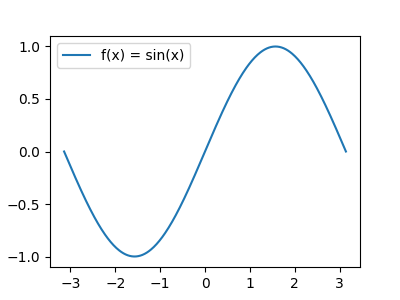
\includegraphics{images/sinus.png}
	\caption{Die  Sinusfunktion.}
\end{figure} 

\subsubsection{Lernen eines Models mit 2 Fuzzy Sets und 1 Ablauf}

Anfangend lasse ich das Model einen Lauf durchzuführen. Wobei hier wichtig zu erwähnen ist, dass eine Iteration und ein Lauf nicht das selbe ist. Iteration im stochastischen Verfahren bedeutet, dass ein Element aus der Datenmenge verarbeitet wurde und ein Lauf - dass alle Elemente erarbeitet sind. Also heißt es für unsere Laufzeit, dass das Model bereits nach einem Lauf 400 Iterationen ausgeführt hat. Die 400 Epochen haben ca. 1.16s gebraucht, wenn wir MF-Typ 0 verwenden. Bei dem MF-Typ 2 werden etwa 0.3s gespart - ca. 0.86s Lerndauer. Die Ergebnisse aus beiden Lerngänge werden unten in zwei Grafiken (\ref{2Sets400_Stoch_0} und \ref{2Sets400_Stoch_1}) zuerst und dann Daten in einer Tabelle gegeben.

\begin{figure}[htbp]\label{2Sets400_Stoch_0}
	\centering
	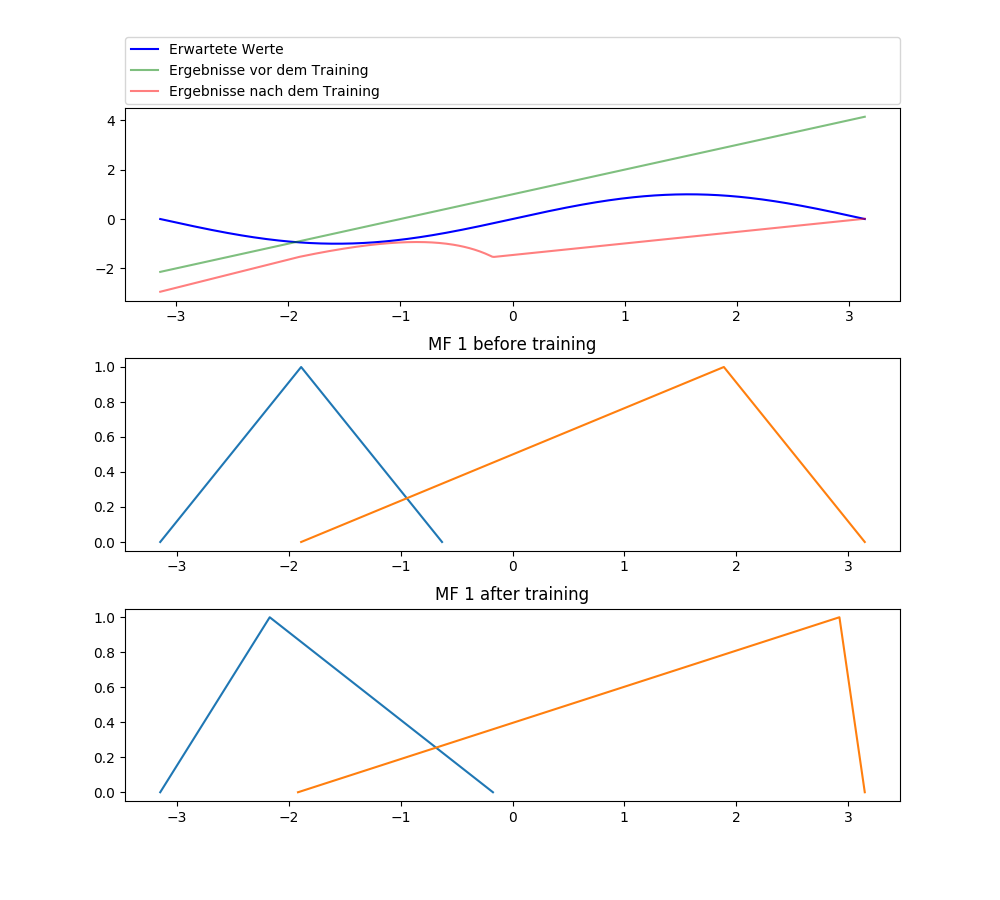
\includegraphics[width=0.75\textwidth]{images/sinus/Stochastic/sinus 1 Input 2 Sets 400 Epochs Stochastic Gradient Descent two equations mf.png}
	\caption{Zwei Fuzzy-Sets, 400 Iterationen, MF-Typ 0}
\end{figure}



\begin{figure}[htbp]\label{2Sets400_Stoch_1}
	\centering
	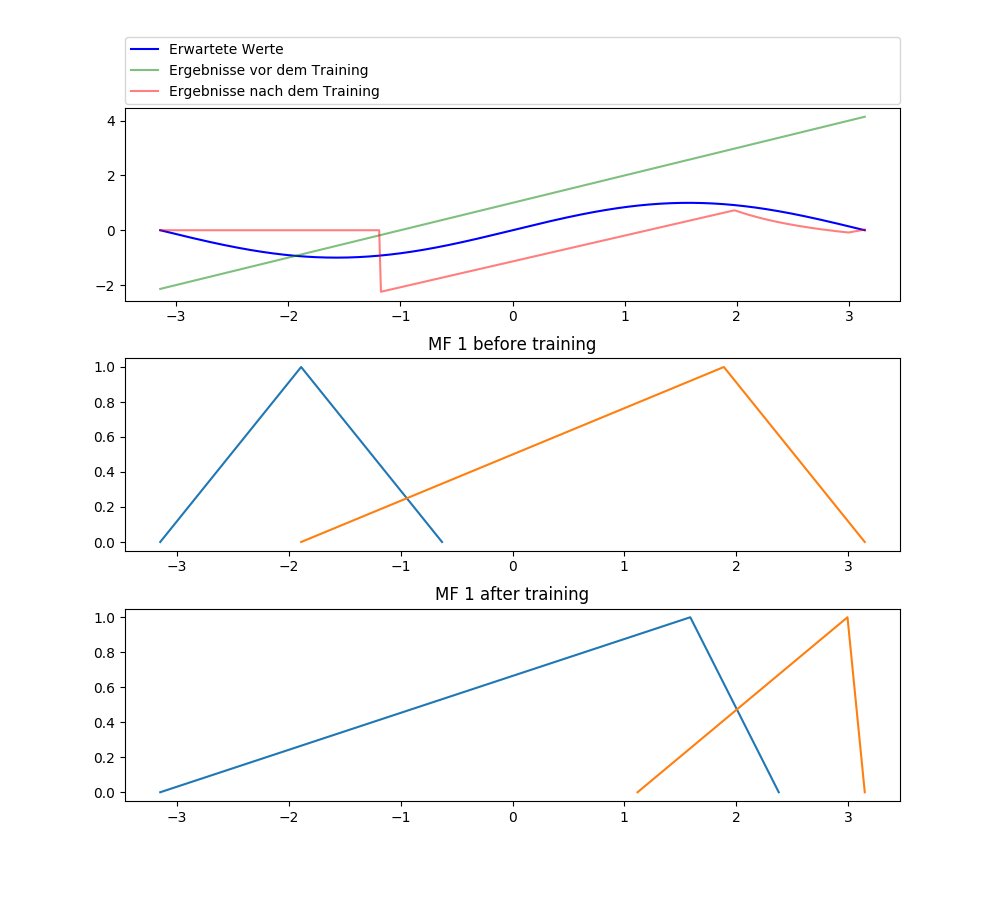
\includegraphics[width=0.75\textwidth]{images/sinus/Stochastic/sinus 1 Input 2 Sets 400 Epochs Stochastic Gradient Descent one equation mf.png}
	\caption{Zwei Fuzzy-Sets, 400 Iterationen, MF-Typ 1}
\end{figure}

Aus der beiden Abbildungen ist schon nach einem Lauf große Änderungen zu erkennen. In den Abbildungen sidn die obersten Grafiken besonders wichtig. Jedoch aus der zweiten Abbildung ist in der Grafik ein Fehler zu erkennen. Da hat die Funktion im Bereich zwischen -3.2 und -1.2 den 0-Wert. Dieses Fehler scheint weiter in den folgenden Testfällen aufzutauchen, aber verschwindet bei den Mini-Batch- und Batch-Lernverfahren. Interessanterweise erhalten wir zwei unterschiedlichen Endergebnisse, obwohl beide Zugehörigkeitsfunktionen die selbe Funktion berechnen. Man erkennt an den Grafiken weiter, dass die Fuzzy-Sets anders gestalltet sind.

In der Tabelle unten ist die Fehlerrate und die Laufzeit abzulesen.

\begin{center}
	\begin{tabular}{ | p{3cm} | l | l | p{3cm} | p{3cm} |}
		\hline
		Type & Time & Error & Gradient Type & MF Type \\ \hline
		sinus 1 Input 2 Sets 400 Epochs Stochastic Gradient Descent two equations mf&1.1651129310000004s&1.8500861&Stochastic Gradient Descent&two equations mf
		 \\ \hline
		sinus 1 Input 2 Sets 400 Epochs Stochastic Gradient Descent one equation mf&0.8567342689999995s&0.74594057&Stochastic Gradient Descent&one equation mf
		 \\ \hline
	\end{tabular}
\end{center}

Die interessantesten Spalten aus der Tabelle sind \textit{Time} und \textit{Error}. Die Zahlen deuten, dass MF-Typ 1 die bessere Vorgehensweise sein soll. Jedoch ist das wegen des Fehlers nicht ganz richtig.

Als letztes sind noch die Konklusionsfunktionen der beiden Lernabläufe.

% mf-type 1
%a_0 [[ 0.64128985]
%[-1.45790108]]
%a_y: [[1.14182867]
%[0.46766532]]

% mf-type 2
%a_0 [[-1.14182764]
%[-2.1789615 ]]
%a_y: [[0.94000338]
%[0.35914132]]

\begin{align}
	\begin{split}\label{mf_0:1}
		y_{mft0_1}(x) = 0.64128985 + 1.14182867\cdot x \\
		y_{mft0_2}(x) = -1.45790108 + 0.46766532\cdot x
	\end{split} \\	
	\begin{split}\label{mf_1:1}
	y_{mft1_1}(x) = -1.14182764 - 0.94000338\cdot x \\
	y_{mft1_2}(x) = -2.1789615 + 0.35914132\cdot x
	\end{split}	
\end{align}

Aus der Konklusionsfunktionen kann man keine Rückschlüsse ziehen. Die Endkurven sind ähnlich, aber das ist kein Wunder, da beide Modelle versuchen, die selbe Funktion zu lernen. 

\subsubsection{Lernen eines Models mit 2 Fuzzy Sets und 10 Abläufe}\label{m2fs10ab}

Der nächste Test endet in 10 Läufe. Die Zwei Tests zeigen keine positiven Ergebnisse. Die Grafiken für die zwei MF-Typen sind sehr Unterschiedlich. Es werden insgesammt vier Tausend Iterationen pro Test durchgeführt, was etwa 7.3s und 6.9s für MF-Typ-0 und MF-Typ-1 entsprechend dauert. Die Abbildungen \ref{2Sets400_Stoch_0} und \ref{2Sets400_Stoch_1} stellen die Ergebnisse der Tests dar.

\begin{figure}[htbp]\label{2Sets4000_Stoch_0}
	\centering
	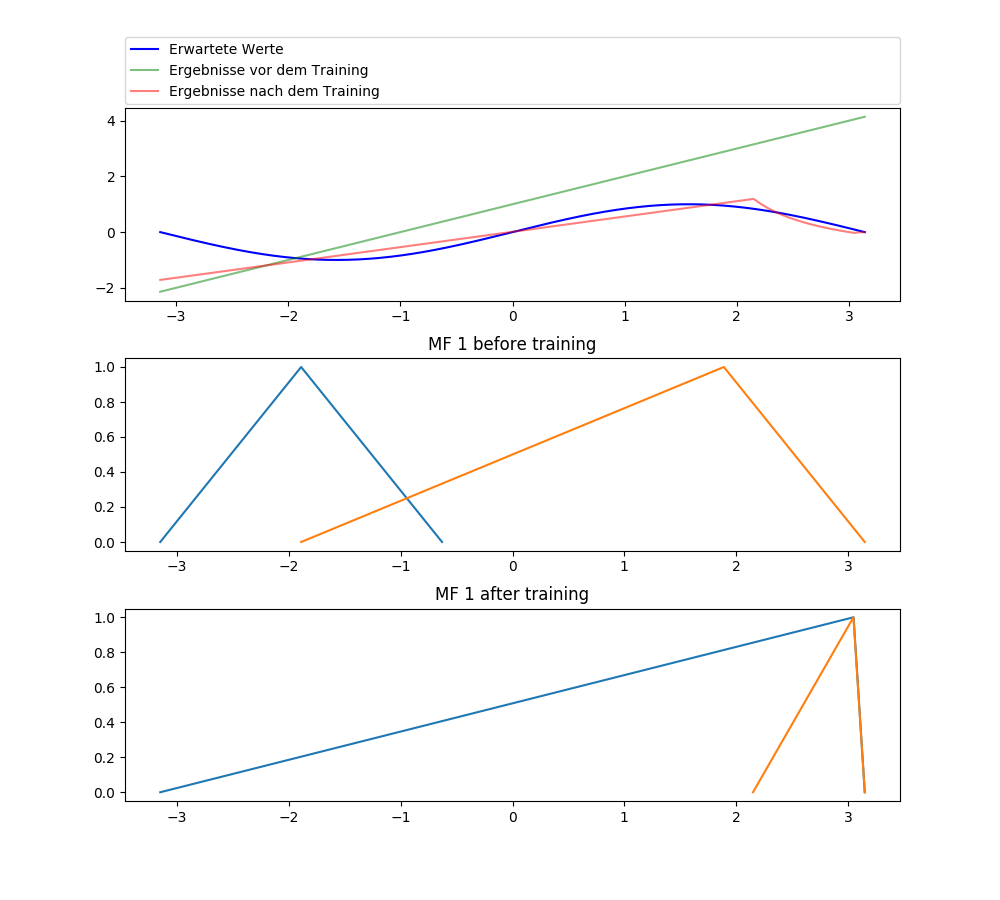
\includegraphics[width=0.75\textwidth]{images/sinus/Stochastic/sinus 1 Input 2 Sets 4000 Epochs Stochastic Gradient Descent two equations mf.png}
	\caption{Zwei Fuzzy-Sets, 4000 Iterationen, MF-Typ 0}
\end{figure}
\begin{figure}[htbp]\label{2Sets4000_Stoch_1}
	\centering
	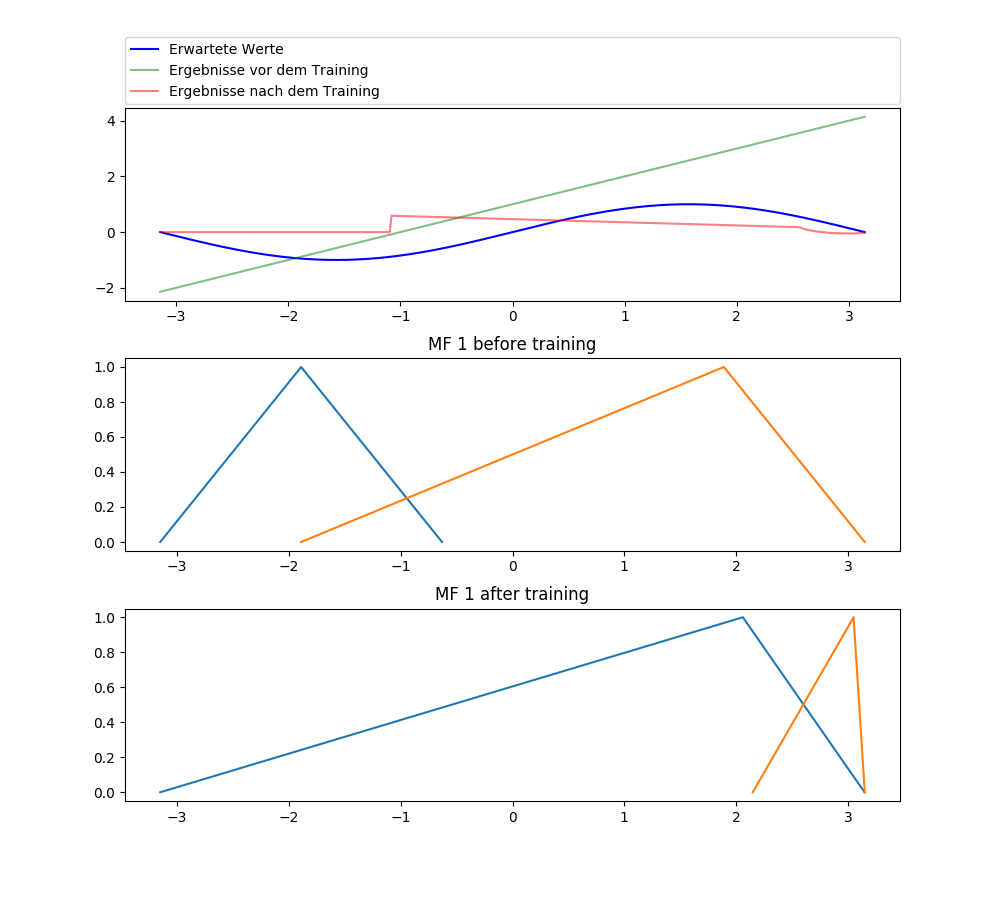
\includegraphics[width=0.75\textwidth]{images/sinus/Stochastic/sinus 1 Input 2 Sets 4000 Epochs Stochastic Gradient Descent one equation mf.png}
	\caption{Zwei Fuzzy-Sets, 4000 Iterationen, MF-Typ 1}
\end{figure}

In der zweiten Abbildung ist wieder das Fehler in der Berechnung zu bemerken. Das Fehler ergibt sich daraus, dass die Katete der gelbe Zugehörigkeitsfunktion zu lang ist. Was bei kleinen X-Werten dazu führt, dass der rechte Teil der Maximumoperation in der Gleichung \ref{mf_typ1} negativ wird.

Die Konklusionsfunktionen sind für beide Modelle gegeben.
% one equation / MF-Type 0
%a_0 [[ 0.01042824]
%[-1.28822409]]
%a_y: [[ 0.54973926]
%[-0.15157128]]

% one equation / MF-Type 1
%a_0 [[ 0.46553119]
%[-1.52831088]]
%a_y: [[-0.11269253]
%[ 0.44669464]]

\begin{align}
	\begin{split}\label{mf_0:10}
		y_{mft1_1}(x) = 0.01042824 + 0.54973926\cdot x \\
		y_{mft1_2}(x) = -1.28822409 - 0.15157128\cdot x
	\end{split} \\	
	\begin{split}\label{mf_1:10}
		y_{mft2_1}(x) = 0.46553119 - 0.11269253\cdot x \\
		y_{mft2_2}(x) = -1.52831088 + 0.44669464\cdot x
	\end{split}	
\end{align}

Im folgenden Fall gibt es wieder keine Ähnlichkeit zwischen den Konklusionsfunktionen der beiden Modelle.

Die Zeiten und Name als auch die Fehlerrate für beide Modell sind in der Tabelle unten angegeben. Daraus können zwei Schlüsse gezogen werden.

\begin{center}
	\begin{tabular}{ | p{3cm} | l | l | p{3cm} | p{3cm} |}
		\hline
		Type & Time & Error & Gradient Type & MF Type \\ \hline
		sinus 1 Input 2 Sets 4000 Epochs Stochastic Gradient Descent two equations mf&7.308665848s&0.21568511&Stochastic Gradient Descent&two equations mf
		\\ \hline
		sinus 1 Input 2 Sets 4000 Epochs Stochastic Gradient Descent one equation mf&6.9275327529999995s&0.50803167&Stochastic Gradient Descent&one equation mf\\ \hline
	\end{tabular}
\end{center}

In der Tabelle können den Fehler und die Laufzeit ausgelesen werden. Anhand der Daten aus dieser Tabelle lässt sich sagen, dass die Berechnung für Modelle des Typs MF-1 kürzer ist, aber Typ 0 Modelle besser lernen.

\subsubsection{Lernen eines Models mit 8 Fuzzy Sets und 10 Abläufe}\label{m8fs10ab}
Im folgenden Testfall ist zu untersuchen, wie wird die Laufzeit beieinflußt, wenn sich die Anzahl der Fuzzymengen erhöht. Im Folgenden Unterkapitel wird der Test mit \textbf{8} Mengen ausgeführt.

Die Ergebnissgrafiken sind zunächst gegeben (\ref{8Sets4000_Stoch_0} und \ref{8Sets4000_Stoch_1}).

\begin{figure}[htbp]\label{8Sets4000_Stoch_0}
	\centering
	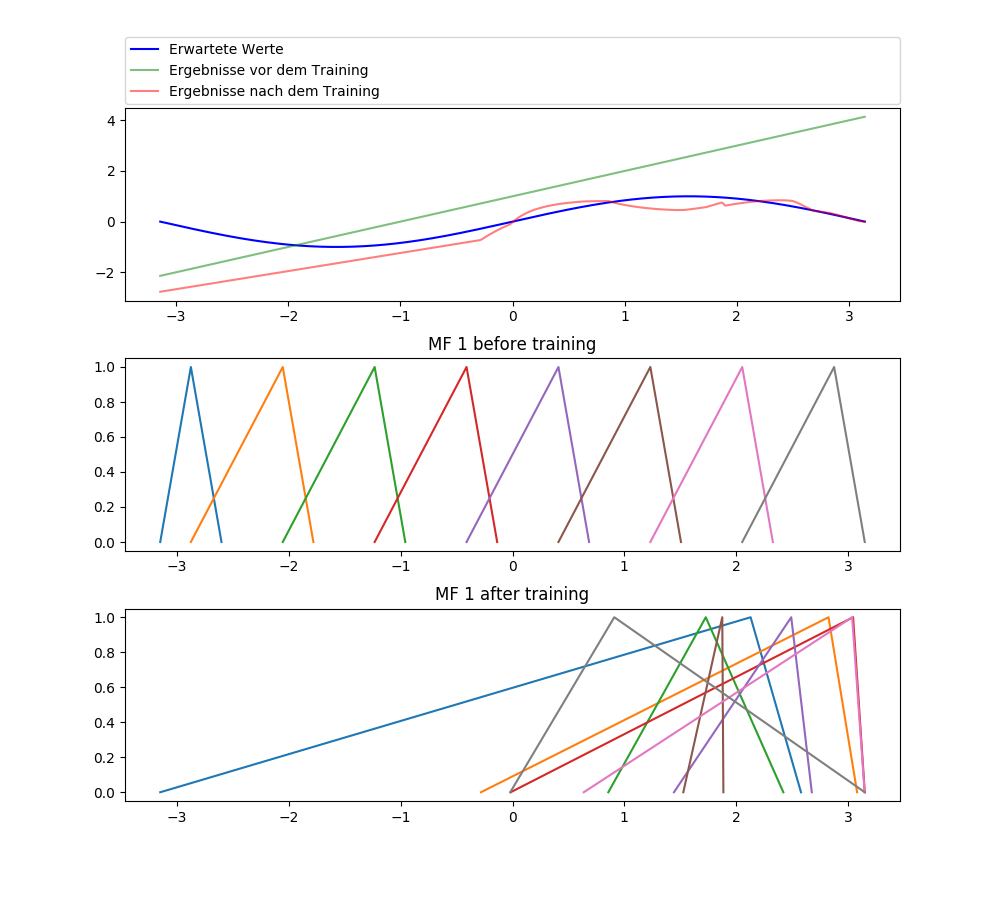
\includegraphics[width=0.75\textwidth]{images/sinus/Stochastic/sinus 1 Input 8 Sets 4000 Epochs Stochastic Gradient Descent two equations mf.png}
	\caption{Acht Fuzzy-Sets, 4000 Iterationen, MF-Typ 0}
\end{figure}
\begin{figure}[htbp]\label{8Sets4000_Stoch_1}
	\centering
	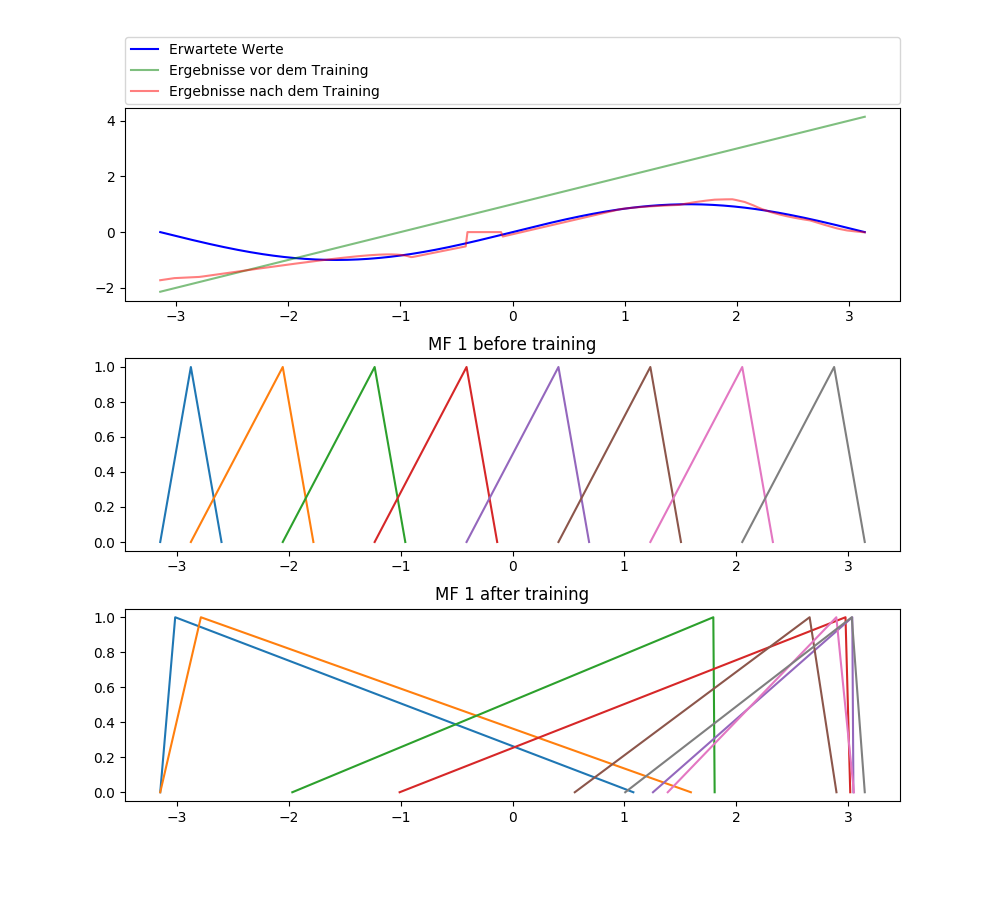
\includegraphics[width=0.75\textwidth]{images/sinus/Stochastic/sinus 1 Input 8 Sets 4000 Epochs Stochastic Gradient Descent one equation mf.png}
	\caption{Acht Fuzzy-Sets, 4000 Iterationen, MF-Typ 1}
\end{figure}

An den Abbildugen erkennt man, dass mit etwas mehr Fuzzy-Mengen, die Funktion lässt sich besser lernen. Man sieht auch große Unterschiede in der Art der gelernten Fuzzymengen. Es ist zu bemerken, dass alle ab dem zweiten Fuzzyset in der ersten Abbildung in die zweite Hälfte der Wertebereich vollgestopft werden. Während in der zweite Abbildung ab dem dritten Fuzzyset. Das ist nur deswegen geschehen, weil bei dem Lernen immer Einzelelemente aus der Datenmenge gezogen werden. Üblicherweise werden bei Lernen immer die betroffenen Parametern nach jeder Iteration angepasst. Also die erste Menge wird als erstes angesprochen und angepasst. Da der linke Parameter nicht geändert werden kann, bedeutet das, dass nur der Mittel- und rechten Grenzparameter nach rechts geschoben werden. Dies erklärt die Vollstopfung am rechten Rand der Wertenbereich.

Die Ergebnisse sind in Tabelle \ref{tab8_4000St} abzulesen.

\begin{center}\label{tab8_4000St}
	\begin{tabular}{ | p{3cm} | l | l | p{3cm} | p{3cm} |}
		\hline
		Type & Time & Error & Gradient Type & MF Type \\ \hline
		sinus 1 Input 8 Sets 4000 Epochs Stochastic Gradient Descent two equations mf&17.413568215999998&0.80348945&Stochastic Gradient Descent&two equations mf \\ \hline
		sinus 1 Input 8 Sets 4000 Epochs Stochastic Gradient Descent one equation mf&14.525632421000001&0.21442673&Stochastic Gradient Descent&one equation mf\\ \hline
	\end{tabular}
\end{center}

Aus der Tabelle die Ergebnisse zeigen, dass der zweite Test deutlich schneller und akkurater lernt. Auf der zweiten Abbildung ist eine Stuffe im Mittleren Bereich zu erkennen, wo sich der Fehler zeigt. Es ist zu lesen, dass das Typ 1 \textit{3} Sekunden schneller ist. Man sieht auch, dass das Verfahren deutlich näher an dem Sollfunktion ist als Typ 0.

Ich gebe die Konklusionsfunktionen nur informative an. Daran können keine weitere Rückschlüsse genannt werden. 
% MF-Typ 0
%a_0 [[-0.5235794 ]
%[ 2.93676464]
%[-3.65265173]
%[ 2.85619127]
%[ 0.1644323 ]
%[-0.92605422]
%[ 0.26038533]
%[ 0.63168423]]
%a_y: [[ 0.71489089]
%[-0.78074253]
%[ 1.63942728]
%[-0.87280814]
%[ 0.55701768]
%[ 1.26660038]
%[-0.12738553]
%[-0.15357252]]
\begin{align}
\begin{split}\label{8mf_0:10}
y_{mft1_1}(x) = -0.5235794 + 0.71489089\cdot x \\
y_{mft1_2}(x) = 2.93676464 - 0.78074253\cdot x \\
y_{mft1_3}(x) = -3.65265173 + 1.63942728\cdot x \\
y_{mft1_4}(x) = 2.85619127 - 0.87280814\cdot x \\
y_{mft1_5}(x) = 0.1644323 + 0.55701768\cdot x \\
y_{mft1_6}(x) = -0.92605422 + 1.26660038\cdot x \\
y_{mft1_7}(x) = 0.26038533 - 0.12738553\cdot x \\
y_{mft1_8}(x) = 0.63168423 - 0.15357252\cdot x
\end{split} \\
% MF-Typ 1
%a_0 [[ 0.46676819]
%[-0.17691342]
%[-0.07739224]
%[ 1.28046489]
%[-1.72202347]
%[ 1.398913  ]
%[ 0.06231506]
%[-0.04088159]]
%a_y: [[ 0.41699012]
%[ 0.80520989]
%[ 0.93785577]
%[-0.94272644]
%[ 0.71823673]
%[ 0.30636544]
%[-0.17987376]
%[-0.28006114]]
\begin{split}\label{8mf_1:10}
y_{mft1_1}(x) = 0.46676819 + 0.41699012\cdot x \\
y_{mft1_2}(x) = -0.17691342 + 0.80520989\cdot x \\
y_{mft1_3}(x) = -0.07739224 + 0.93785577\cdot x \\
y_{mft1_4}(x) = 1.28046489 - 0.94272644\cdot x \\
y_{mft1_5}(x) = -1.72202347 + 0.71823673\cdot x \\
y_{mft1_6}(x) = 1.398913 + 0.30636544\cdot x \\
y_{mft1_7}(x) = 0.06231506 - 0.17987376\cdot x \\
y_{mft1_8}(x) = -0.04088159 - 0.28006114\cdot x
\end{split}	
\end{align}

%\begin{tabular}
%	
%\end{tabular}
\subsection{Fazit}

Die beschriebenen Testfälle sind nicht die Einzigen. Am Ende der Arbeit werden alle Tests zusammen mit einer großen Tabelle angehängt. Aus allen Tests bin ich zu der Überzeugung gekommen, dass die Berechnung mit MF-Typ 0 richtiger ist, auch wenn die Fehlerrate schlechter ist. Ich bin genau zu der Überzeugung gekommen, weil nämmlich eine Berechnung mit MF-Typ 1 nur für symmetrische Fuzzymengen geeignet ist. Da aber in meiner Ausarbeitung das nicht immer der Fall ist, werden ich in den nächsten Kapiteln nur mit der zwei Gleichungmethode vorgehen. Außerdem die schnellere Laufzeit des Typ 1 Models erklärt daraus, dass bei dem MF-Typ 0 eine zusätzliche Berechnung durchzuführen ist (zwei Gleichungen).

Es ist sehr wichtig zu erwähnen, dass das Lernen mit mehr Mengen etwa \textbf{1,3} mal länger dauert. Während eine verdopplung in Iterationen, auch die doppelte von Laufzeit erfordert, was auch zu erwarten ist.

Hier ist schwehr die beste Konfiguration fürs Lernen zu nennen. Ich würde sogar sagen, dass das Lernen mit dem stochastischen Verfahren ungeeignet ist.

\section{Lernen der Sinusfunktion mit Mini-Batch Gradient Descent}

In diesem Kapitel handelt es sich um die Mini-Batch Gradient Descent. Das Verfahren wurde am Anfang dieses \ref{mini_batch}. Kapitel  vorgestellt. Ziel der folgenden Untersuchungen ist es zu zeigen, welche die beste Konfiguration fürs Model ist. Außerdem werden im Fazit die beiden Verfahren (Mini-Batch und Stochastic) verglichen. 

\subsubsection{Lernen der Sinusfunktion mit 2 Fuzzy-Sets und 1 Ablauf}

Begonnen werden soll mit dem Lernen der Funktion mit zwei Fuzzymengen und der Ablauf verläuft über einen Gang. Die Testbeschreibung beinhaltet nur den MF-Typ 0.

\begin{figure}[htbp]\label{abb2fs5itmb}
	\centering
	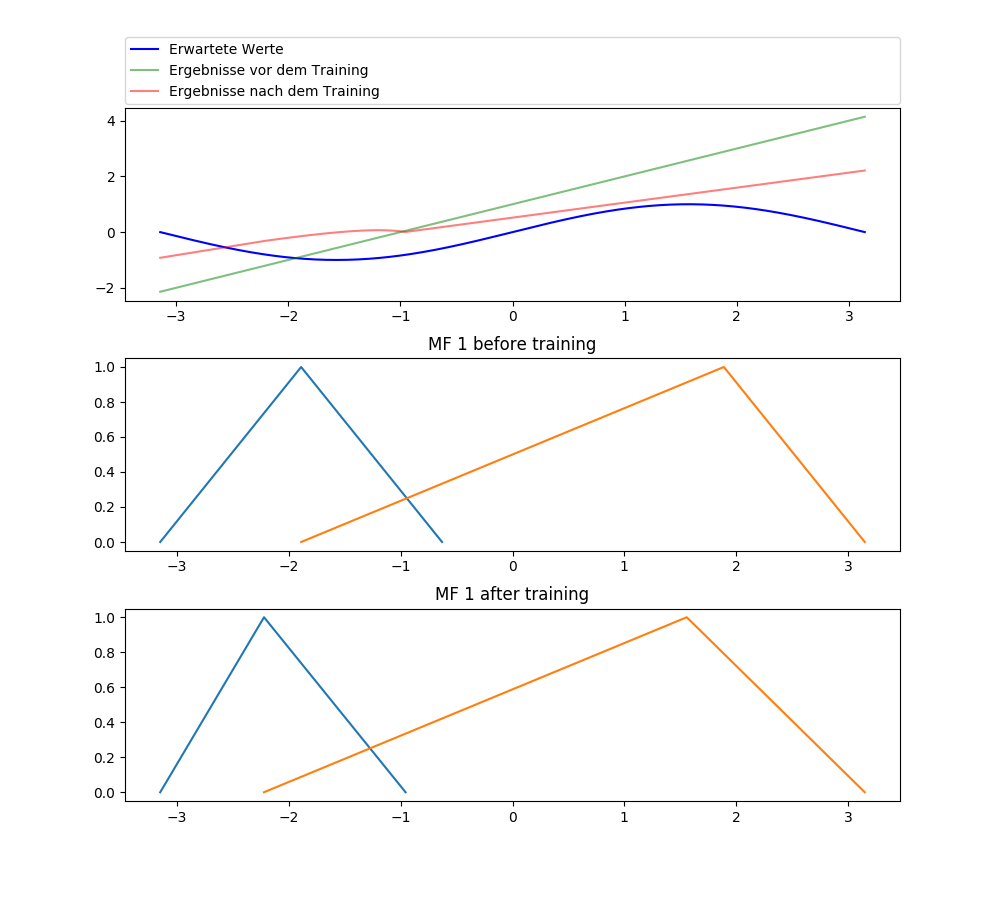
\includegraphics[width=0.75\textwidth]{images/sinus/Mini-Batch/sinus 1 Input 2 Sets 5 Epochs Mini-Batch Gradient Descent two equations mf.png}
	\caption{2 Fuzzy-Sets, 5 Iterationen, MF-Typ 0}
	\label{2mini_batch5:0}
\end{figure}

In der Grafik sieht man keine große Änderung in den Fuzzy-Sets als auch in der Ergebnissfunktion. Das ist jedoch kein Wunder, da es nur 5 Iterationen durchgeführt werden. Der Dauer dieser Test entspricht 14 ms.

Zur Abgleich habe ich die Ergebnisse aus dem vorrigen Unterkapitel und diesen Test
angegben.
\begin{center}\label{tab2_5MB}
	\begin{tabular}{ | p{3cm} | l | l | p{3cm} | p{3cm} |}
		\hline
		Type & Time & Error & Gradient Type & MF Type \\ \hline
		sinus 1 Input 2 Sets 5 Epochs Mini-Batch Gradient Descent two equations mf&0.1438041160000001&0.70317644&Mini-Batch Gradient Descent&two equations mf \\ \hline
		sinus 1 Input 2 Sets 400 Epochs Stochastic Gradient Descent two equations mf&1.1651129310000004s&1.8500861&Stochastic Gradient Descent&two equations mf
		\\ \hline
	\end{tabular}
\end{center}

Die Fehlerrate ist wie erwartet sehr hoch, jedoch viel kleiner als der Stochastic. Außerdem ist die Endfunktion sehr ähnlich wie aus der Vorrigenkapitel (siehe \ref{2Sets400_Stoch_0}). Man erkennt aus den beiden Abbildungen, dass in Abbildung \ref{2Sets400_Stoch_0} die Funktion im Negativen Y-Bereich liegt, während die \ref{2mini_batch5:0} nur in dem Abschnit zwischen -3.2 bis ungefähr -1. 

Es ist eine schnellere Laufzeit als der stochastische Verfahren zu erkennen. Die kürze Lerndauer erklärt sich dadurch, da der Datensatz schneller abgearbeitet wird - in Fünf Schritte, im Vergleich zu Vierhundert. Es ist zu erwarten, dass nach 400 Iterationen das Modell noch besser (niedrigere Fehlerrate) sein soll. Im nächsten Kapitel wird diese Aussage untersucht.

Schließlich gebe ich die Konklusionsfunktion für das Model.

%MF-Typ 0
%a_0 [[1.12589365]
%[0.51933658]]
%a_y: [[0.65193717]
%[0.53854825]]

\begin{align}
\begin{split}\label{2mini_mf_0:0}
y_{mft1_1}(x) = 1.12589365 + 0.65193717\cdot x \\
y_{mft1_2}(x) = 0.51933658 + 0.53854825\cdot x
\end{split}
\end{align}

Zwischen die Funktionen \ref{2mini_mf_0:0} und \ref{mf_0:1} ist in die Erste Gleichung zu erkennen, dass sich die Parametern ihre Plätze getauscht haben. Ein weiterer Unterschied ist, dass es keine negativen Parametern gelernt wurden.

%MF-Typ 1
%a_0 [[0.95071704]
%[0.51425419]]
%a_y: [[0.70936966]
%[0.52004189]]

\subsubsection{Lernen der Sinusfunktion mit 2 Fuzzy-Sets und 10 Ablauf}
Als nächstes ist das Model mit 10 Abläufe zu betrachten. Die Frage, die in diesem Kapitel beantwortet werden soll, ist, ob das Lernen mit Teile der Datenmenge wirklich besser ist. Deswegen vergleiche ich die Ergebnisse von Kapitel \ref{m2fs10ab} mit den aus diesem. 

Eine Ergebnissabbildung wird unten gezeichnet.

\begin{figure}[htbp]
	\centering
	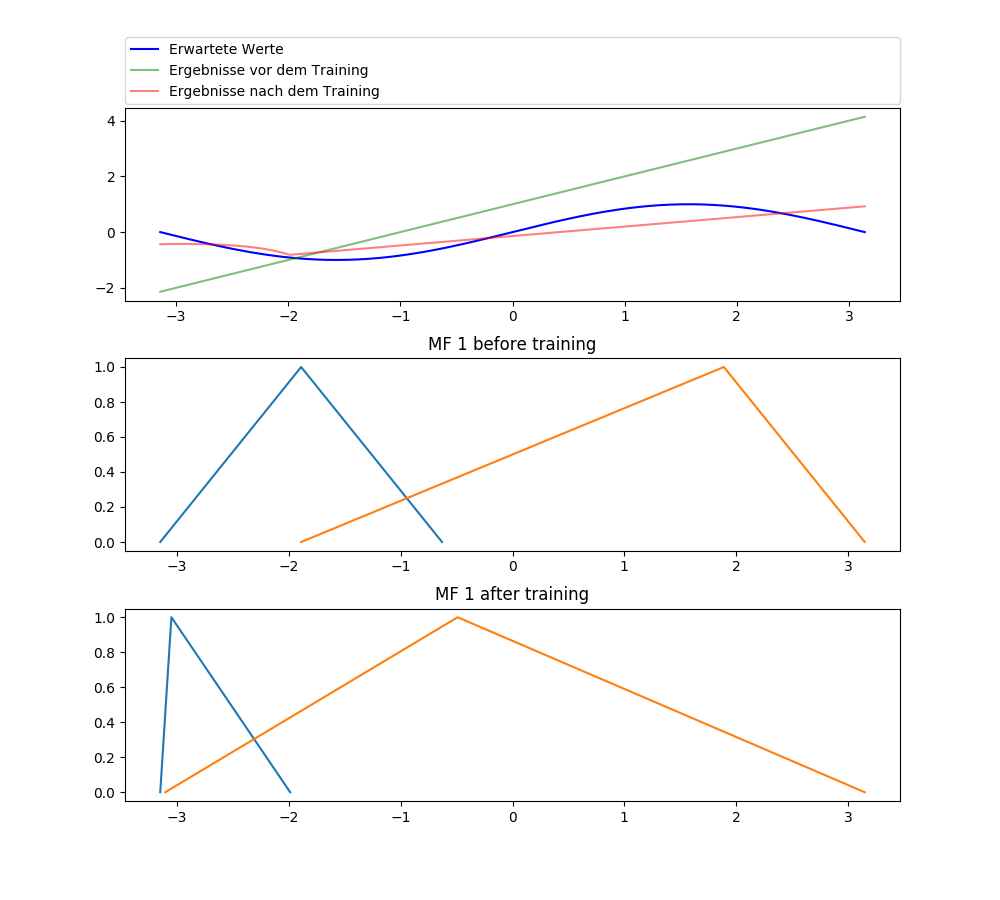
\includegraphics[width=0.75\textwidth]{images/sinus/Mini-Batch/sinus 1 Input 2 Sets 50 Epochs Mini-Batch Gradient Descent two equations mf.png}
	\caption{2 Fuzzy-Sets, 50 Iterationen, MF-Typ 0}
	\label{2mini_batch50:0}
\end{figure}

Die Fuzzy-Mengen haben eine deutlich größere Änderung im Vergleich zu dem aus vorrigen Kapitel Modell unterlegen. Das Lernen hat 0.2s gedauert. Das ist etwa 30 Mal schneller als der stochastische Verfahren. Die Daten für beide Modelle stehen mit Fehlerrate und Dauer in der Tabelle unten.

\begin{center}\label{tab2_50MB}
	\begin{tabular}{ | p{3cm} | l | l | p{3cm} | p{3cm} |}
		\hline
		Type & Time & Error & Gradient Type & MF Type \\ \hline
		sinus 1 Input 2 Sets 50 Epochs Mini-Batch Gradient Descent two equations mf&0.2727800499999997&0.1554767&Mini-Batch Gradient Descent&two equations mf\\ \hline
		sinus 1 Input 2 Sets 4000 Epochs Stochastic Gradient Descent two equations mf&7.308665848s&0.21568511&Stochastic Gradient Descent&two equations mf
		\\ \hline
	\end{tabular}
\end{center}

Man erzielt nicht nur ein schnelleres Lernen mit dem Mini-Batch Verfahren, man erhält auch ein besseres Lernen. Die Fehlerrate ist von 0.22 um 50\% auf 0.16 abgestiegen.

Zum Schluss sind die Inferenzfunktionen für das Modell gegeben.

% mftyp 0
%a_0 [[ 0.58986986]
%[-0.14078197]]
%a_y: [[0.32787314]
%[0.3395195 ]]

\begin{align}
	y_{mft1_1}(x) = 0.58986986 + 0.32787314\cdot x \\
	y_{mft1_2}(x) = -0.14078197 + 0.3395195\cdot x
\end{align}

\subsubsection{Lernen der Sinusfunktion mit 2 Fuzzy-Sets und 1000 Abläufe}
In diesem Abschnitt wird das Ergebnis aus dem Test mit 1000 Abläufe vorgestellt. Das Model verfügt weiterhin über 2 Fuzzymengen und wird mit MF-Typ 0 gelernt. Die Abbildung \ref{2mini_batch1000:0} berichtet das Endergebniss.

Bei dieser Konfiguration lernt das Model mit nur einer Zugehörigkeitsgleichung auch sehr erfolgreich. Die Abbildungen der beiden Tests sind sehr ähnlich. Die Grafiken \ref{2mini_batch1000:1} und \ref{2mini_batch1000:0} sind untereinander angegeben.

\begin{figure}[htbp]\label{2mini_batch1000:0}
	\centering
	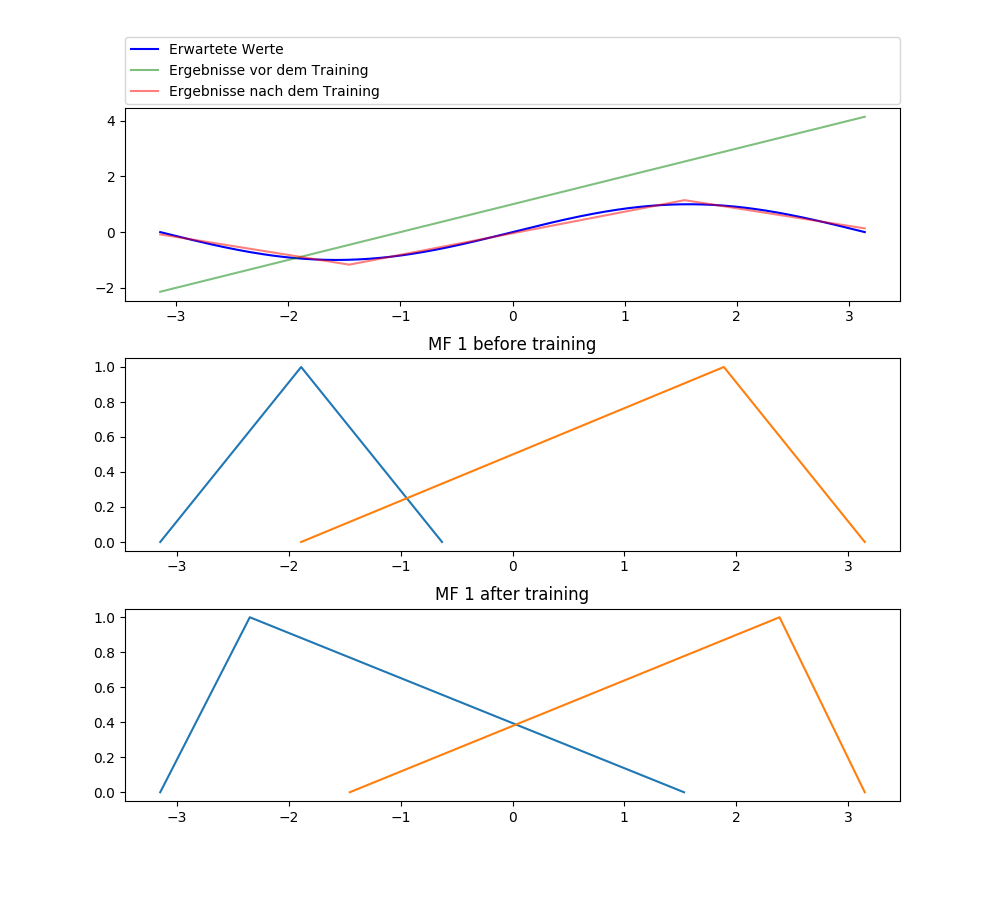
\includegraphics[width=0.75\textwidth]{images/sinus/Mini-Batch/sinus 1 Input 2 Sets 5000 Epochs Mini-Batch Gradient Descent two equations mf.png}
	\caption{2 Fuzzy-Sets, 1000 Iterationen, MF-Typ 0}
\end{figure}
\begin{figure}[htbp]\label{2mini_batch1000:1}
	\centering
	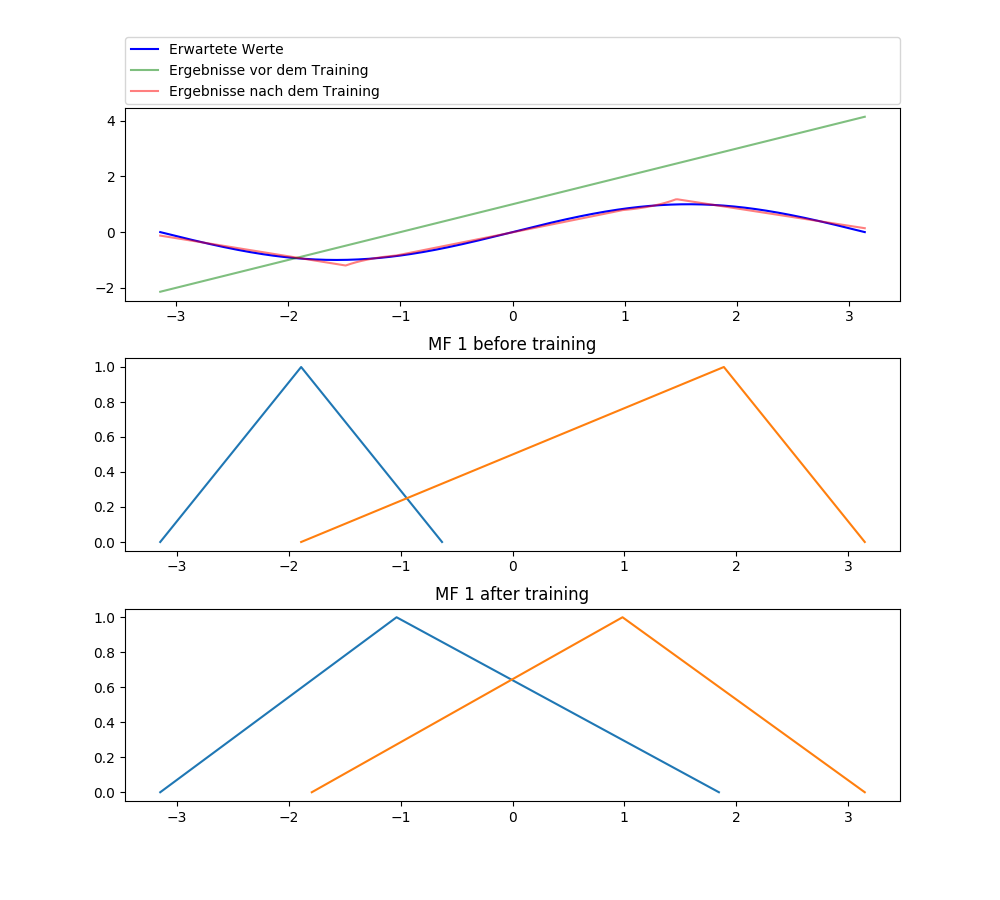
\includegraphics[width=0.75\textwidth]{images/sinus/Mini-Batch/sinus 1 Input 2 Sets 5000 Epochs Mini-Batch Gradient Descent one equation mf.png}
	\caption{2 Fuzzy-Sets, 1000 Iterationen, MF-Typ 0}
\end{figure}

Das Endergebniss aus der zweiten Abbildung scheint auf den ersten Blick besser zu sein. Der größte Unterschied liegt in den Fuzzymengen. Die gelernten Fuzzysets überlappen zur unterschiedlichen Stuffen. Die Mengen in der zweiten Abbildung überschneiden sich deutlich mehr. Die Reichweite ist in dem Fall etwa 4 Skalawerten und auf der ersten Abbildung sind es ungefähr 3. Die zusätzlichen Daten, die in der Tabelle unten zu finden sind, beantworten die Frage, welches Model besser ist.

\begin{center}\label{tab2_1000MB}
	\begin{tabular}{ | p{3cm} | l | l | p{3cm} | p{3cm} |}
		\hline
		Type & Time & Error & Gradient Type & MF Type \\ \hline
		sinus 1 Input 2 Sets 5000 Epochs Mini-Batch Gradient Descent two equations mf&11.761141329s&0.006521431&Mini-Batch Gradient Descent&two equations mf \\ \hline
		sinus 1 Input 2 Sets 5000 Epochs Mini-Batch Gradient Descent one equation mf&10.697818779s&0.0048954873&Mini-Batch Gradient Descent&one equation mf \\ \hline
	\end{tabular}
\end{center}

Die Vermutung war richtig. Das zweite Model ist mit etwa 0,02 Einheiten besser und mit einer Sekunde schneller. Die Frage taucht jetzt auf, wo liegt der Unterschied zwischen die beiden Modellen? Ist es wegen des Unterschieds in der Fuzzymengen, oder sind die Inferenzfunktionen einfach unterschiedlich? Die Antwort wird erst klar, wenn die Gleichungen für die Konklusionen betrachtet werden.



% Endfunktion mftyp 0
%a_0 [[-2.10781751]
%[ 2.1163349 ]]
%a_y: [[-0.64453965]
%[-0.63109723]]

% Endfunktion mftyp 1
%a_0 [[-2.17036302]
%[ 2.09081218]]
%a_y: [[-0.65073889]
%[-0.62095912]]

\begin{align}
\begin{split}\label{2mf_0:1000}
y_{mft1_1}(x) = -2.10781751 - 0.64453965\cdot x \\
y_{mft1_2}(x) = 2.1163349 - 0.63109723\cdot x
\end{split} \\	
\begin{split}\label{2mf_1:1000}
y_{mft2_1}(x) = -2.17036302 - 0.65073889\cdot x \\
y_{mft2_2}(x) = 2.09081218 - 0.62095912\cdot x
\end{split}	
\end{align}

Die Antwort auf die Frage lautet, dass der Unterschied liegt in den Fuzzymengen. Die Gleichungen sind bis auf der zweiten Dezimalzahl identisch. Die Tatsache, dass die Werte überhaupt so ähnlich sind, ist ein Wunder.

Wenn man die beiden Ergebnisse betrachtet, erkennt man wie schlecht das stochastische Verfahren lernt. Allein mit \textbf{10} Abläufe bei den Stochastischen Tests hat man fast die selbe Anzahl an Iterationsschritten und trotzdem ist das Ergebniss \textbf{100} mal schlechter (die Fehlerrate ist gemeint).

\section{Lernen der Parabelfunktion}

Die Struktur dieser Kapitel ähnelt dem aus Vorherigen. In Laufe der Ausarbeitung bin ich einer sehr interessanten Frage gestoßen. Ich wollte untersuchen, ob das Vorzeichen der Trainingsdaten einen Einfluß auf das Lernen hat. Um das zu überprüfen, habe ich die Parabelfunktion verändert, so dass die positiven X-Werten einnimmt. In einem der Abschnitte unterscheide ich zwischen die beiden Funktion.

Die eigentlichen Funktionen, die gelernt werden müssen, sind in zwei Grafiken zu sehen:
\begin{figure}
	\centering
	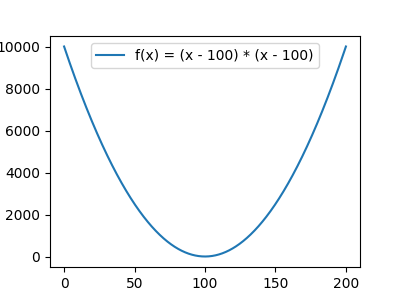
\includegraphics{images/parabola_positive.png}
	\caption{Die quadratische Funktion.}
\end{figure}
\begin{figure}
	\centering
	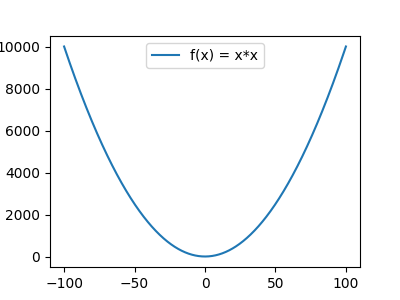
\includegraphics{images/parabola.png}
	\caption{Die quadratische Funktion.}
\end{figure}

Auf der ersten Grafik erkennt man, dass die X-Werten nur Positive sind. Ich werde jetzt einige Ergebnisse vorstellen und zeigen, ob die ANFIS-Modelle die Funktionen gleich lernen.

\subsection{Lernen der Parabelfunktion mit Mini-Batch Gradient Descent}

Zuerst betrachten wir zwei Modelle, die das Lernen über 10 Abläufe, bzw. 50 Iterationen, durchführen:
\begin{figure}[htbp]
	\centering
	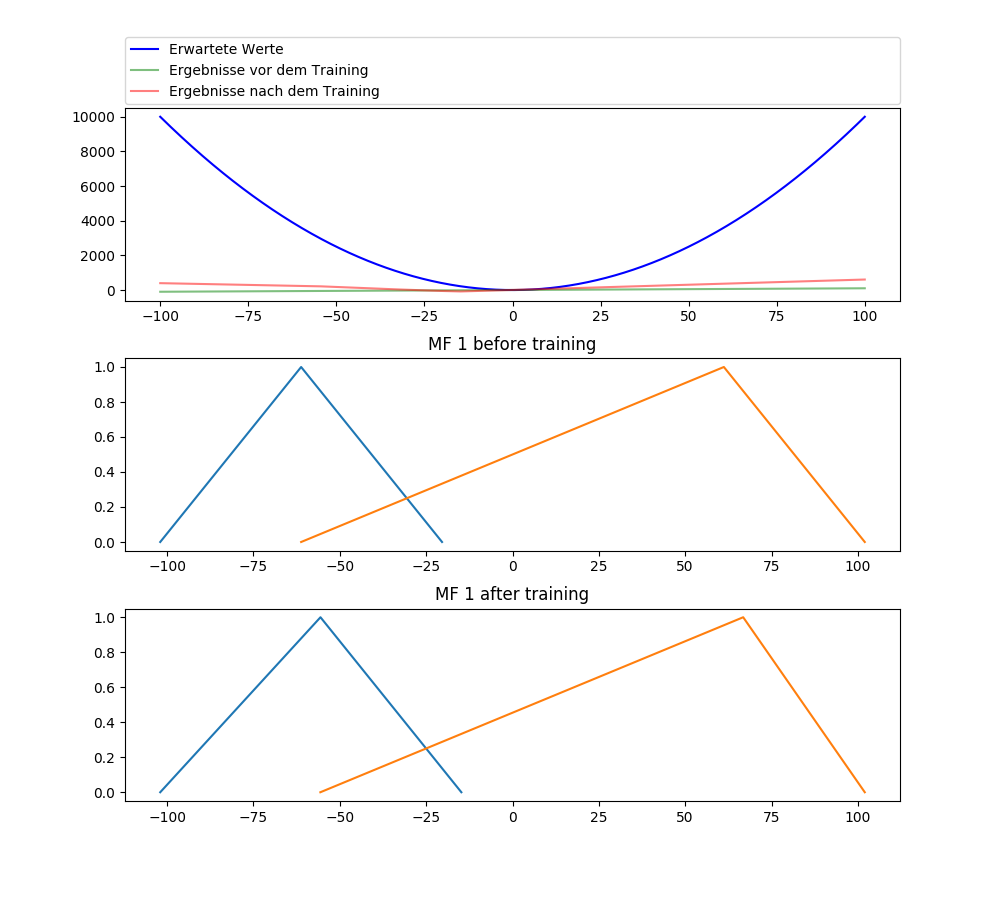
\includegraphics[width=0.75\textwidth]{images/parabola_1000/Mini-Batch/parabola_1000 1 Input 2 Sets 50 Epochs Mini-Batch Gradient Descent two equations mf.png}
	\caption{2 Fuzzy-Sets, 50 Iterationen, MF-Typ 0}
\end{figure}
\begin{figure}[htbp]
	\centering
	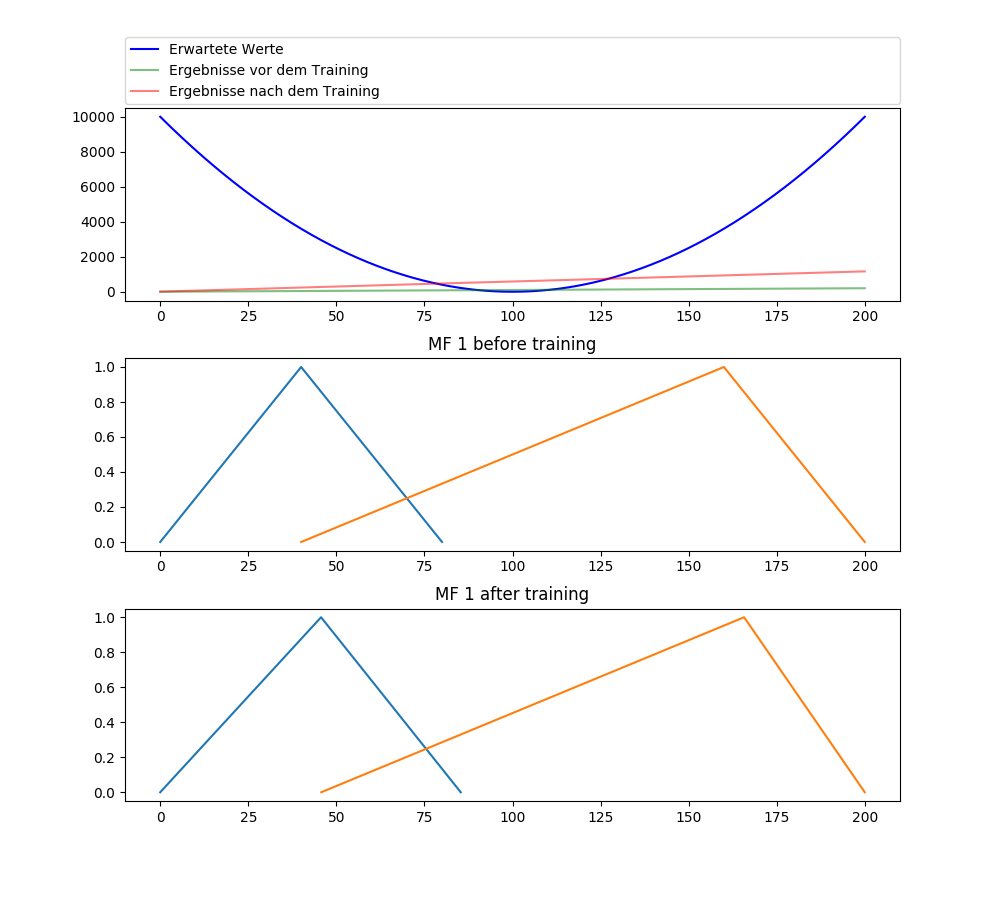
\includegraphics[width=0.75\textwidth]{images/parabola_positive/Mini-Batch/parabola_positive 1 Input 2 Sets 50 Epochs Mini-Batch Gradient Descent two equations mf.png}
	\caption{2 Fuzzy-Sets, 50 Iterationen, MF-Typ 0 mit nur Positiven X-Werte}
\end{figure}

In diesem Fall ist die Anzahl der Durchläufe viel zu klein, damit wesentliche Ergebnisse geliefert werden. Man erkennt, dass in der ersten Grafik die Enden der Kurve nach oben geschoben sind, währen gegen der 0 Punkt tief liegt. In der zweiten Grafik erkennt man keine Kurve wirklich, sondern eine Gerade, die sich ein wenig von der Anfangsgerade gehoben hat. Betrachten wir nun die nummerische Unterschiede in der Tabelle \ref{par_tab1_50MB}:

\begin{center}\label{par_tab1_50MB}
	\begin{tabular}{ | p{3.1cm} | l | l | p{3cm} | p{3cm} |}
		\hline
		Type & Time & Error & Gradient Type & MF Type \\ \hline
		parabola\_1000 & 0.27263559800000037 & 17675046.0 & Mini-Batch Gradient Descent & two equations mf
		 \\ \hline
		parabola\_positive & 0.26520074800000026 & 16615864.0 & Mini-Batch Gradient Descent & two equations mf
		 \\ \hline
	\end{tabular}
\end{center} 

Aus der Grafik erkennt man, dass das ``positive'' Modell sowohl schneller als auch ``richtiger'' ist. Die Bilder würden deuten, dass das ``normale'' Model besser ist, aber die nummerischen Daten sagen, dass das andere Modelle das bessere wäre. Aus den Erkenntnissen lässt sich keine Schlüsse ziehen. Aus dem nächsten Beispiel stellt sich jedoch heraus, welche Aufgabe besser gelernt werden kann.

Als nächsten werden wir die zwei Modellen 1000 Mal laufen lassen, das würde heißen das es insgesammt 5000 Iterationen durchgeführt werden. Die weiteren Konfigurationen verbleiben gleich. Zuerst werden die Grafiken aus den beiden Tests gegeben:

\begin{figure}[htbp]
	\centering
	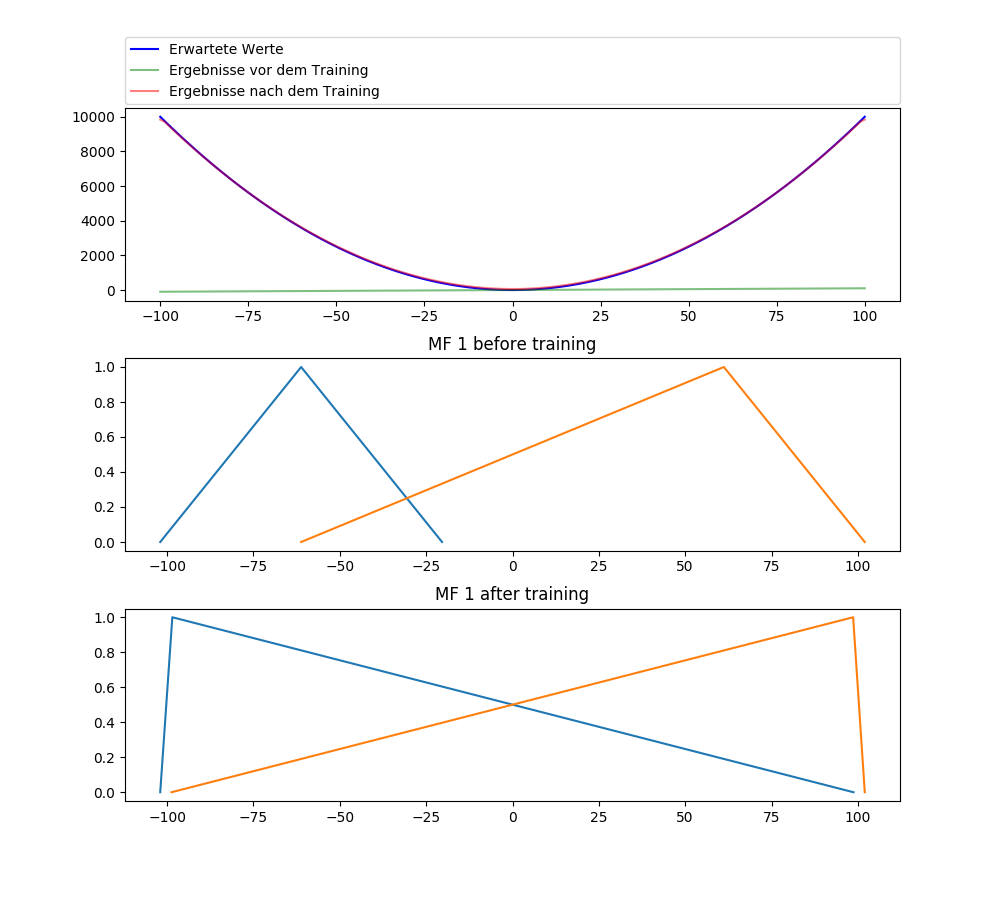
\includegraphics[width=0.75\textwidth]{images/parabola_1000/Mini-Batch/parabola_1000 1 Input 2 Sets 5000 Epochs Mini-Batch Gradient Descent two equations mf.png}
	\caption{2 Fuzzy-Sets, 5000 Iterationen, MF-Typ 0}
\end{figure}
\begin{figure}[htbp]
	\centering
	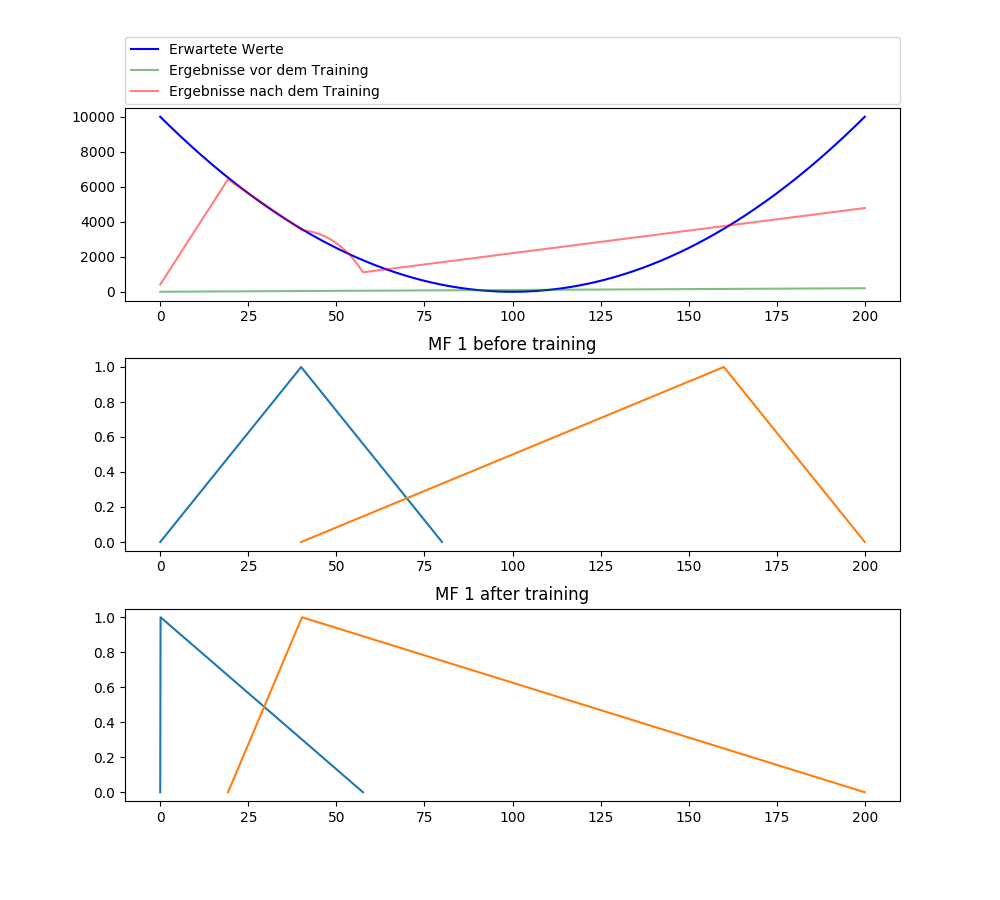
\includegraphics[width=0.75\textwidth]{images/parabola_positive/Mini-Batch/parabola_positive 1 Input 2 Sets 5000 Epochs Mini-Batch Gradient Descent two equations mf.png}
	\caption{2 Fuzzy-Sets, 5000 Iterationen, MF-Typ 0 mit nur Positiven X-Werte}
\end{figure}

Aus den Grafiken ist zu lesen, dass das Modell mit positiven und negativen Trainingsdaten schneller den Optimalzustand erreicht als das positve Modell. Außerdem nach 5000 Iterationen ist das Netz sehr gut trainiert. Es ist zu erwarten, dass die nummerische Daten auch für das erste Beispiel sprechen.

\begin{center}\label{par_tab1_5000MB}
	\begin{tabular}{ | p{3.1cm} | l | l | p{3cm} | p{3cm} |}
		\hline
		Type & Time & Error & Gradient Type & MF Type \\ \hline
		parabola\_1000 & 12.538009995&1682.427&Mini-Batch Gradient Descent&two equations mf
		\\ \hline
		parabola\_positive & 12.474743275000002&5956089.5&Mini-Batch Gradient Descent&two equations mf
		\\ \hline
	\end{tabular}
\end{center}

Wie auch schon aus den Grafiken ersichtlich geworden ist, dass das gemischte Modell etwas geeigneter für das Lernen der Parabel Funktion ist. Auch die nummerischen Daten sprechen dafür, dass dies der Fall ist. Es besteht ein riesiger Unterschied in den Fehlerraten der beiden Testfälle.


\subsection{Fazit}

